%%%%%%%%%%%%%%%%%%%%%%%%%%%%%%%%%%%%%%%%%
% Sullivan Business Report
% LaTeX Template
% Version 1.0 (May 5, 2022)
%
% This template originates from:
% https://www.LaTeXTemplates.com
%
% Author:
% Vel (vel@latextemplates.com)
%
% License:
% CC BY-NC-SA 4.0 (https://creativecommons.org/licenses/by-nc-sa/4.0/)
%
%%%%%%%%%%%%%%%%%%%%%%%%%%%%%%%%%%%%%%%%%

%----------------------------------------------------------------------------------------
%	CLASS, PACKAGES AND OTHER DOCUMENT CONFIGURATIONS
%----------------------------------------------------------------------------------------

\documentclass[
	a4paper, % Paper size, use either a4paper or letterpaper
	12pt, % Default font size, the template is designed to look good at 12pt so it's best not to change this
	%unnumberedsections, % Uncomment for no section numbering
]{include/CSSullivanBusinessReport}

\addbibresource{include/sample.bib} % BibLaTeX bibliography file

%-----------------------------------------------------------------------
%	REPORT INFORMATION
%-----------------------------------------------------------------------
\reporttitle{Propuesta de Servicios Secretaria de la Alcaldía de
Bogotá} % The report title to appear on the title page and page headers, do not create manual new lines here as this will carry over to page headers

\reportsubtitle{A professional layout featuring a large margin\\ and examples of typical business report content} % Report subtitle, include new lines if needed

\reportauthors{Template created by:\\\smallskip Vel (vel@latextemplates.com)} % Report authors/group/department, include new lines if needed

\reportdate{\today} % Report date, include new lines for additional information if needed

\rightheadercontent{
\includegraphics[width=3cm]{./include/creodocs_logo.pdf}} % The content in the right header, you may want to add your own company logo or use your company/department name or leave this command empty for no right header content

\def\tightlist{}
%------------------------------------------------------------------------

\begin{document}

%------------------------------------------------------------------------
%	TITLE PAGE
%------------------------------------------------------------------------
\thispagestyle{empty} % Suppress headers and footers on this page

\begin{fullwidth} % Use the whole page width
	\vspace*{-0.075\textheight} % Pull logo into the top margin
	
	\hfill
\includegraphics[width=5cm]{./include/creodocs_logo.pdf} % Company logo

	\vspace{0.15\textheight} % Vertical whitespace

	\parbox{0.9\fulltextwidth}{\fontsize{50pt}{52pt}\selectfont\raggedright\textbf{\reporttitle}\par} % Report title, intentionally at less than full width for nice wrapping. Adjust the width of the \parbox and the font size as needed for your title to look good.
	
	\vspace{0.03\textheight} % Vertical whitespace
	
	{\LARGE\textit{\textbf{\reportsubtitle}}\par} % Subtitle
	
	\vfill % Vertical whitespace
	
	{\Large\reportauthors\par} % Report authors, group or department
	
	\vfill\vfill\vfill % Vertical whitespace
	
	{\large\reportdate\par} % Report date
\end{fullwidth}

\newpage

%----------------------------------------------------------------------------------------
%	DISCLAIMER/COPYRIGHT PAGE
%----------------------------------------------------------------------------------------
\thispagestyle{empty} % Suppress headers and footers on this page

\begin{twothirdswidth} % Content in this environment to be at two-thirds of the whole page width
	\footnotesize % Reduce font size
	
	\subsection*{Disclaimer}

	Lorem ipsum dolor sit amet, consectetur adipiscing elit. Praesent porttitor arcu luctus, imperdiet urna iaculis, mattis eros. Pellentesque iaculis odio vel nisl ullamcorper, nec faucibus ipsum molestie. Sed dictum nisl non aliquet porttitor. Etiam vulputate arcu dignissim, finibus sem et, viverra nisl. Aenean luctus congue massa, ut laoreet metus ornare in. Nunc fermentum nisi imperdiet lectus tincidunt vestibulum at ac elit.
	
	\subsection*{Copyright}
	
	\textcopyright~[Year] [Company] 
	
	Copyright notice text\ldots In hac habitasse platea dictumst. Curabitur mattis elit sit amet justo luctus vestibulum. In hac habitasse platea dictumst. Pellentesque lobortis justo enim, a condimentum massa tempor eu. Ut quis nulla a quam pretium eleifend nec eu nisl. Nam cursus porttitor eros, sed luctus ligula convallis quis.
	
	\subsection*{Contact}
	
	Address Line 1\\
	Address Line 2\\
	Address Line 3
	
	Business Number 123456
	
	Contact: name@company.com
	
	\vfill % Push the following down to the bottom of the page
	
	\subsubsection*{Changelog}
	
	\scriptsize % Reduce font size further
	
	\begin{tabular}{@{} L{0.05\linewidth} L{0.15\linewidth} L{0.6\linewidth} @{}} % Column widths specified here, change as needed for your content
		\toprule
		v1.0 & 20XX-02-05 & Lorem ipsum dolor sit amet, consectetur adipiscing elit. Praesent porttitor arcu luctus, imperdiet urna iaculis, mattis eros.\\
		v1.1 & 20XX-02-27 & Pellentesque iaculis odio vel nisl ullamcorper, nec faucibus ipsum molestie.\\
		v1.2 & 20XX-03-15 & Sed dictum nisl non aliquet porttitor.\\
		\bottomrule
	\end{tabular}
\end{twothirdswidth}

\newpage

%----------------------------------------------------------------------------------------
%	TABLE OF CONTENTS
%----------------------------------------------------------------------------------------
\begin{twothirdswidth} % Content in this environment to be at two-thirds of the whole page width
	\tableofcontents % Output the table of contents, automatically generated from the section commands used in the document
\end{twothirdswidth}

\newpage

%----------------------------------------------------------------------------------------
%	SECTIONS
%----------------------------------------------------------------------------------------

\newpage

\section{Información del
Documento}\label{sec:informaciuxf3n-del-documento}

Esta es la doc del grupo.

\subsection{Versión del Documento}\label{sec:versiuxf3n-del-documento}

\begin{quote}
\end{quote}

Versión actual 1.1434244 - repository\_dispatch - Sun, 22 Jun 2025
21:38:39 -0500

\subsection{Control de Cambios}\label{sec:control-de-cambios}

Historia de cambios del documento.

1.15600e5 - Compilación para entrega: accion-contd (4c3c821) - Wed, 18
Jun 2025 21:33:07 +0000

1.4aeee1c - commitmsj--gh\_action - Wed, 18 Jun 2025 16:10:36 -0500

1.b377c5d - Compilación para entrega: accion-contd (4a47ca2) - Wed, 18
Jun 2025 21:08:29 +0000

1.a73be24 - commitmsj--gh\_action - Wed, 18 Jun 2025 16:07:12 -0500

\subsubsection{Realizado Por}\label{sec:realizado-por}

(creador)

\subsubsection{Revisado Por}\label{sec:revisado-por}

(revisor), Arquitectura de Aplicaciones

\newpage

\section{Servicios de Ingeniería Arquitectura de Aplicaciones Secretaria
de la Alcaldía de
Bogotá}\label{sec:servicios-de-ingenieruxeda-arquitectura-de-aplicaciones-secretaria-de-la-alcalduxeda-de-bogotuxe1}

\subsection{Descripción de la
Propuesta}\label{sec:descripciuxf3n-de-la-propuesta}

\begin{quote}
\end{quote}

Consultoría de ingeniería y mejoramiento del canal bancario textual
Whatsapp del Secretaria de la Alcaldía de Bogotá, con extensión a
sistemas externos, legados y proveedores tecnológicos relacionados con
la arquitectura del canal.

\subsection{Detalles Técnicos de la
Propuesta}\label{sec:detalles-tuxe9cnicos-de-la-propuesta}

\begin{quote}
\end{quote}

Esta propuesta contienen los siguientes componentes técnicos.

\begin{itemize}
\tightlist
\item
  Metas del proyecto
\item
  Alcance
\item
  Métodos
\item
  Entregables
\item
  Plan de trabajo
\item
  Propuesta económica
\item
  Consideraciones y restricciones
\end{itemize}

\subsection{Metas de la Propuesta}\label{sec:metas-de-la-propuesta}

\begin{quote}
\end{quote}

\begin{enumerate}
\def\labelenumi{\arabic{enumi}.}
\tightlist
\item
  \textbf{Diagnóstico}. Hallazgos relevantes de la arquitectura del
  Arquitectura de Aplicaciones. Presentar puntos de cambios relevantes
  resultado del análisis de la arquitectura de solución actual del canal
  de banca Whatsapp (chat) del Secretaria de la Alcaldía de Bogotá
  categorizados en varias perspectivas, como la funcional, técnica y
  operativa.
\item
  \textbf{Hoja de Ruta}. Lista de cambios y gestión de cambios de la de
  la arquitectura del Arquitectura de Aplicaciones**. Desarrollar la
  hoja de ruta de los cambios derivados del objetivo no. 1, Hallazgos
  relevantes de la arquitectura, con una priorización planteada mediante
  criterio críticos de factibilidad e impacto a Secretaria de la
  Alcaldía de Bogotá.
\end{enumerate}

\subsection{Alcance}\label{sec:alcance}

\begin{quote}
\end{quote}

\begin{enumerate}
\def\labelenumi{\arabic{enumi}.}
\tightlist
\item
  Diagnóstico. Evaluación de la arquitectura del Arquitectura de
  Aplicaciones del Secretaria de la Alcaldía de Bogotá que resulta en
  puntos de cambios accionables de la arquitectura del Arquitectura de
  Aplicaciones.
\item
  Diseño de hoja de ruta de transformación. Planteamiento de transición
  de la arquitectura del Arquitectura de Aplicaciones mediante lista de
  cambios priorizados sobre la arquitectura del canal.
\end{enumerate}

\subsubsection{Exclusiones del
Alcance}\label{sec:exclusiones-del-alcance}

La presenta propuesta no incluye:

\begin{enumerate}
\def\labelenumi{\arabic{enumi}.}
\tightlist
\item
  Por restricciones de tiempo, la actual propuesta no incluye análisis
  ni recomendaciones de diseño a arquitectura distintas a las del
  Arquitectura de Aplicaciones.
\item
  No incluye plan de capacidad ni proyección de uso infraestructura
  futura de la arquitectura del Arquitectura de Aplicaciones.
\item
  No incluye la provisión de infraestructura para las soluciones
  derivadas de este proyecto.
\item
  No incluye soporte ni mantenimiento posterior a la realización de este
  proyecto.
\end{enumerate}

\subsection{Método Propuesto}\label{sec:muxe9todo-propuesto}

\begin{quote}
\end{quote}

\begin{enumerate}
\def\labelenumi{\arabic{enumi}.}
\tightlist
\item
  Planificación. Período inicial de definición y acuerdos de los
  objetivos puntuales de las evaluación de la arquitectura del
  Arquitectura de Aplicaciones.
\item
  Preparación y Alistamiento. Lista de chequeo de recursos, personas y
  procesos relacionadas con las vistas de arquitectura del Arquitectura
  de Aplicaciones, como las vistas funcional, técnica, despliegues, y
  otras.
\item
  Definición. Confirmación del diseño de los escenarios de evaluación de
  la arquitectura del Arquitectura de Aplicaciones. Identificación de
  otras dependencias entre escenarios.
\item
  Diagnóstico. Profundización del detalle de la información, ejecución
  de los métodos seleccionados para la evaluación de la arquitectura, y
  documentación reproducible de los resultados.
\item
  Verificación. Contrastar el resultado preliminar de los escenarios de
  evaluación de la arquitectura del Arquitectura de Aplicaciones contra
  el método de evaluación.
\item
  Divulgación de Resultados y Entregables. (luego de la verificación)
  Explicar el resultado general de la evaluación de los escenarios de la
  arquitectura del Arquitectura de Aplicaciones y discrepancias con
  umbrales de aceptación.
\item
  Diseño de Hoja de Ruta. Preparación, alistamiento y priorización de
  las transiciones de la arquitectura del Arquitectura de Aplicaciones
  (hoja de ruta).
\item
  Divulgación de Resultados y Entregables Finales. Compilación de
  artefactos, documentación técnica y divulgación de conocimiento del
  resultado de diagnóstico y de la hoja de ruta priorizada de la
  arquitectura del Arquitectura de Aplicaciones.
\end{enumerate}

\begin{figure}
\centering
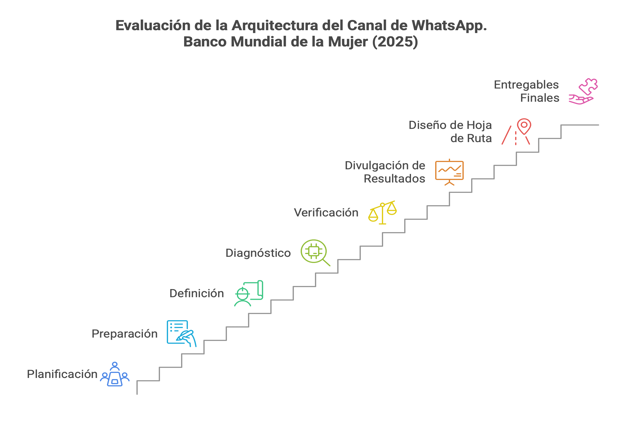
\includegraphics{images/02.1c.Metodo.png}
\caption{02.1c.Metodo. \emph{Fuente: Propuesta servicios de ingeniería y
evaluación de arquitectura Arquitectura de Aplicaciones Secretaria de la
Alcaldía de Bogotá
(2025)}}\label{fig:id-ecb3efe1a4e14dd389ece75370f1861c}
\end{figure}

\subsection{Entregables de la
Propuesta}\label{sec:entregables-de-la-propuesta}

\begin{quote}
\end{quote}

\begin{enumerate}
\def\labelenumi{\arabic{enumi}.}
\tightlist
\item
  Visión. Definición trabajo arquitecrura
\item
  Arquitectura actual sistemas información
\item
  Arquitectura solución
\item
  Catálogo sistemas información
\item
  Implementación y Migración
\end{enumerate}

\newpage

\section{Aspectos Técnicos de la
Propuesta}\label{sec:aspectos-tuxe9cnicos-de-la-propuesta}

\subsection{Plan de Trabajo}\label{sec:plan-de-trabajo}

\begin{quote}
\end{quote}

El plan de trabajo propuesto consta de dos fases consecutivas que
inician a partir de la aceptación y formalización de la actual
propuesta. La Fase I, llamada en esta propuesta el diagnóstico y
evaluación de la arquitectura; y la Fase II, destinada al diseño de la
hoja de ruta de transformación de la arquitectura del Arquitectura de
Aplicaciones.

En detalle cada fase del proyecto:

\begin{enumerate}
\def\labelenumi{\arabic{enumi}.}
\item
  Día 1 al 15. Diagnóstico y evaluación de la arquitectura del
  Arquitectura de Aplicaciones, incluye planificación, preparación,
  diagnóstico, documentación técnica, y divulgación: estimada en 15 días
  de trabajo.
\item
  Día 16 al 20. Diseño de hoja de ruta de transformación de la
  arquitectura del Arquitectura de Aplicaciones, incluye diseño de hoja
  de ruta, ejecución transiciones, gestión de cambios, documentación
  técnica, divulgación: estimada en 5 días de trabajo.
\end{enumerate}

\subsection{Plazo de Ejecución}\label{sec:plazo-de-ejecuciuxf3n}

Por todo lo anterior, el total de la duración del proyecto es de un (1)
mes laboral.

\begin{figure}
\centering
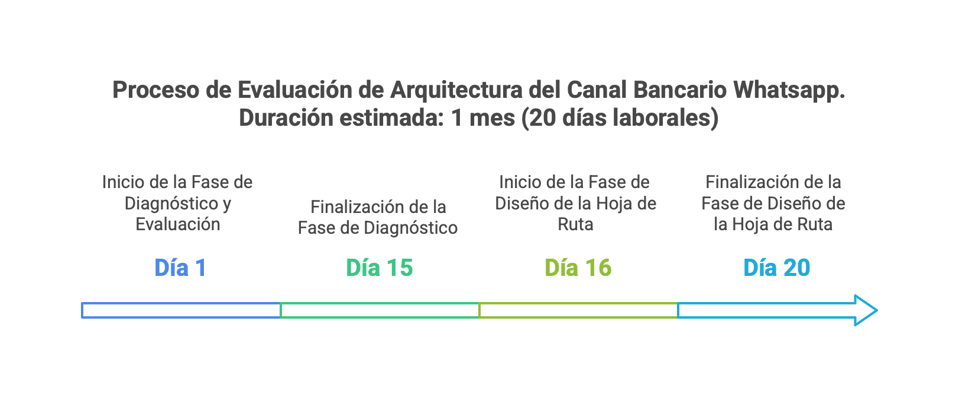
\includegraphics{images/02.1e1.Plan.png}
\caption{02.1e1.Plan. \emph{Fuente: Propuesta servicios de ingeniería y
evaluación de arquitectura Arquitectura de Aplicaciones Secretaria de la
Alcaldía de Bogotá
(2025)}}\label{fig:id-650dca2ba0114dca99ad6302b8ed6dc7}
\end{figure}

\subsection{Propuesta Económica}\label{sec:propuesta-econuxf3mica}

\begin{quote}
\end{quote}

A la presente propuesta, en los términos consignados aquí, le
corresponde la siguiente propuesta económica.

\begin{longtable}[]{@{}
  >{\raggedright\arraybackslash}p{(\columnwidth - 6\tabcolsep) * \real{0.5161}}
  >{\raggedright\arraybackslash}p{(\columnwidth - 6\tabcolsep) * \real{0.1828}}
  >{\raggedright\arraybackslash}p{(\columnwidth - 6\tabcolsep) * \real{0.1505}}
  >{\raggedright\arraybackslash}p{(\columnwidth - 6\tabcolsep) * \real{0.1505}}@{}}
\toprule\noalign{}
\begin{minipage}[b]{\linewidth}\raggedright
Ítem
\end{minipage} & \begin{minipage}[b]{\linewidth}\raggedright
Valor (COP \$/.)
\end{minipage} & \begin{minipage}[b]{\linewidth}\raggedright
IVA (19\%)
\end{minipage} & \begin{minipage}[b]{\linewidth}\raggedright
Total
\end{minipage} \\
\midrule\noalign{}
\endhead
\bottomrule\noalign{}
\endlastfoot
Evaluación y hoja de ruta de arquitectura Arquitectura de Aplicaciones &
\$ 62'000,000 & \$ 11'400.000 & \$ 71'400.000 \\
Descuento del 10\% Cliente Primera Vez & \$ 6.000.000 & \$ 1.140.000 &
\$ 7.140.000 \\
TOTAL & \$ 54.000.000 & \$ 10.260.000 & \$ 64.260.000 \\
\end{longtable}

Nota: los valores del costo de la propuesta se mantienen durante los
siguientes 10 días laborales luego de su presentación a los interesados.

\subsubsection{Forma de Pago de la
Propuesta}\label{sec:forma-de-pago-de-la-propuesta}

\begin{longtable}[]{@{}lll@{}}
\toprule\noalign{}
Pagos & Fracción & Hito del Plan \\
\midrule\noalign{}
\endhead
\bottomrule\noalign{}
\endlastfoot
Primer pago & 50\% & Evaluación de la arquitectura \\
Segundo pago & 50\% & Hoja de Ruta Priorizada \\
\end{longtable}

\subsection{Consideraciones
Importantes}\label{sec:consideraciones-importantes}

\begin{quote}
\end{quote}

\begin{enumerate}
\def\labelenumi{\arabic{enumi}.}
\tightlist
\item
  Forma de pago de la propuesta: 50\% al final del primer entregables,
  50\% al final del segundo entregable.
\item
  Por las restricciones propias de proyecto la ejecución de este
  proyecto requiere apoyo de un ingeniero interno de la empresa,
  dedicado el tiempo convenido entre las partes.
\item
  Las estimaciones de costo, esfuerzo, tiempo, y planeación son
  aproximadas, y representan la intención de la propuesta basada en la
  información conocida por las partes al momento de su realización.
\item
  Las extensiones en los entregables, o cambios a la propuesta se
  acordarán en definiciones y extensiones por separado.
\end{enumerate}

\newpage

\section{Resumen de la Propuesta}\label{sec:resumen-de-la-propuesta}

\subsection{}\label{sec:section}

\begin{quote}
\end{quote}

\begin{itemize}
\tightlist
\item
  El resultado del proyecto es el diagnóstico y la lista de cambios
  priorizados sobre la arquitectura del Arquitectura de Aplicaciones, la
  divulgación de los cambios y la documentación técnica
\item
  La duración del proyecto es de un (1) mes de trabajo (días laborales).
\item
  El equipo de trabajo propuesto será provisto por el proponente.
\item
  El valor económico de la propuesta es \$64.260.000 COP, IVA incluido.
\item
  Esta propuesta no incluye recomendaciones de diseño, intervenciones a
  sistemas distintos de los consignados en el alcance, ni servicios de
  infraestructura, ni soporte posterior al presente proyecto.
\item
  Requiere apoyo de ingenieros y personal interno de la empresa, nivel
  de participación acordado entre las partes.
\item
  Una vez finalizada la ejecución de esta propuesta (no. 1), según
  acuerdo de continuidad, realizaremos una nueva para el desarrollo de
  la solución de los casos consignados en la hoja de ruta (propuesta no.
  1).
\end{itemize}

\subsection{Equipo de Trabajo}\label{sec:equipo-de-trabajo}

\begin{quote}
\end{quote}

El equipo de trabajo requerido para el cumplimiento del alcance, metas y
entregables de la actual propuesta será provisto por el proponente.

Nota Por las restricciones de ejecución usuales en este tipo de
proyectos es requerido apoyo interno de la empresa cliente del
Arquitectura de Aplicaciones. El nivel de participación en el proyecto y
el rol del recurso interno se acuerdan a conveniencia de las partes,
cliente y
proponente.\sidenote{This is a sidenote. This template features a large margin specifically so you can put notes, figures, tables and other things into it as additional material to the main content in the text block.}

Donec in elit ac ante vestibulum rhoncus. Pellentesque ligula tortor, aliquet malesuada nulla tristique vitae. Aliquam mi sem, varius eu pellentesque et, tristique nec quam. Vestibulum pellentesque in dui et venenatis. Sed malesuada elit pellentesque sapien aliquet porta. In at facilisis diam. Duis id ante tellus.\sidenote[][2cm]{This sidenote has been pushed down the page manually with an optional parameter, otherwise it would be right under the one above.} % This first optional argument to a sidenote is the symbol to use (leave this empty for automatic numbering) and the second is the vertical offset (positive is down, negative is up)

In diam libero, vulputate quis accumsan non, auctor in ipsum. Praesent cursus velit eget lacus sodales porta. Proin quis risus ut velit euismod scelerisque ut sed neque. Cras sagittis, dolor ac ullamcorper auctor, tortor dui facilisis diam, at sagittis nisi ipsum a neque. Nullam vel mattis nisi. Ut interdum ut diam at ornare. Nulla ultrices elit justo, vitae tristique massa vulputate sit amet.

\nonumsidenote{
	}Vestibulum erat felis, cursus vitae convallis ac, commodo eu nisi. Nulla facilisi. Mauris dignissim nisi felis, a mollis ex accumsan vel. Suspendisse bibendum vitae nibh in suscipit. Vestibulum et finibus eros. Nulla facilisi. Cras luctus aliquam finibus. In nec justo nec orci malesuada faucibus.

\subsubsection{Subsubsection Title} % Third level section

\begin{fullwidth} % Use the whole page width
	\textit{This is an example of a full width paragraph\ldots} Curabitur id placerat orci. Vivamus pulvinar augue ac feugiat blandit. Donec in ultricies mi. Nam eu lacus ac augue aliquet consectetur. Praesent dui risus, sollicitudin nec felis ut, posuere ultricies dolor. Sed massa nulla, dignissim eget sem sit amet, eleifend fermentum dui. Phasellus consequat sem vel turpis finibus, a aliquam risus malesuada.
\end{fullwidth}

Maecenas consectetur metus at tellus finibus condimentum. Proin arcu lectus, ultrices non tincidunt et, tincidunt ut quam. Integer luctus posuere est, non maximus ante dignissim quis. Nunc a cursus erat. Curabitur suscipit nibh in tincidunt sagittis. Nam malesuada vestibulum quam id gravida. Proin ut dapibus velit. Vestibulum eget quam quis ipsum semper convallis. Duis consectetur nibh ac diam dignissim, id condimentum enim dictum. Nam aliquet ligula eu magna pellentesque, nec sagittis leo lobortis. Aenean tincidunt dignissim egestas. Morbi efficitur risus ante, id tincidunt odio pulvinar vitae.

\paragraph{Paragraph Title} % Fourth level section

Lorem ipsum dolor sit amet, consectetur adipiscing elit. Aliquam auctor mi risus, quis tempor libero hendrerit at. Duis hendrerit placerat quam et semper. Nam ultricies metus vehicula arcu viverra, vel ullamcorper justo elementum. Pellentesque vel mi ac lectus cursus posuere et nec ex.

The section titles below show how multi-line section titles look at the 3 top levels.


%----------------------------------------------------------------------------------------
%	QUOTATIONS
%----------------------------------------------------------------------------------------

\section{Quotations}

Proin mollis urna posuere fringilla. Curabitur finibus, neque vitae vestibulum vestibulum, dolor sapien tincidunt augue, vel porta mauris metus nec mauris. Integer erat magna, porta id erat sed, lacinia volutpat erat. Nulla fermentum tellus arcu, eu iaculis ipsum malesuada aliquam. Duis et lacus maximus, consectetur metus et, eleifend arcu. Vestibulum condimentum diam vitae diam tincidunt viverra.\sidenotequote[-1cm]{\textbf{\LARGE ``}Lorem ipsum dolor sit amet, consectetur adipiscing elit. Praesent porttitor arcu luctus, imperdiet urna iaculis, mattis eros. Pellentesque iaculis odio vel nisl ullamcorper, nec faucibus ipsum molestie.\textbf{''}\\[4pt]\hfill--- John Smith, 1972} % Example margin quotation using the \sidenotequote custom command

\begin{quote}
	\textbf{\LARGE ``}Lorem ipsum dolor sit amet, consectetur adipiscing elit. Praesent porttitor arcu luctus, imperdiet urna iaculis, mattis eros. Pellentesque iaculis odio vel nisl ullamcorper, nec faucibus ipsum molestie. Sed dictum nisl non aliquet porttitor. Etiam vulputate arcu dignissim, finibus sem et, viverra nisl. Aenean luctus congue massa, ut laoreet metus ornare in.\textbf{''}
	
	\hfill--- John Smith, 1972
\end{quote}

Suspendisse tempus odio sit amet volutpat suscipit. Pellentesque ornare libero lacus, non fringilla dolor placerat in. Ut maximus ullamcorper lectus, a pharetra mi sagittis aliquet. Scelerisque augue sed mi fringilla, vel dapibus ligula finibus. Sed ornare velit sem, ac venenatis velit dignissim. Vestibulum ultrices mi at tincidunt condimentum.

%----------------------------------------------------------------------------------------
%	TABLES
%----------------------------------------------------------------------------------------

\section{Table Examples}

This statement automatically references the table below using its label: Table \ref{tab:example}.

%------------------------------------------------

\begin{margintable} % Use the margintable environment for tables to be output to the margin
	\footnotesize % Reduce the font size in the table as space is at a premium
	\caption{Margin table caption.}
	\begin{tabular}{L{0.22\linewidth} C{0.22\linewidth} R{0.25\linewidth}}
		\toprule
		\textbf{Year} & \textbf{Qtr.} & \textbf{Perf.}\\
		\midrule
		20XX & Q1 & 0.5\%\\
		20XX & Q2 & 26.5\%\\
		20XX & Q1 & 35.4\%\\
		20XX & Q4 & 41.3\%\\
		\bottomrule
	\end{tabular}
\end{margintable}

%------------------------------------------------

\begin{table}[H] % [H] forces the table to be output where it is defined in the code (it suppresses floating)
	\caption{Text block table caption.}
	\begin{tabular}{L{0.35\linewidth} L{0.38\linewidth} L{0.16\linewidth}}
		\toprule
		\textbf{Prospect} & \textbf{Industry} & \textbf{Revenue} \\
		\midrule
		Gerlach Inc & Business Development & 3M\\
		Doyle and Sons & Law & 1M\\
		Heathcote Group & Consulting & 12M\\
		Goyette Inc & Advertising & 5M\\
		Holzdeppe GmbH & Manufacturing & 23M\\
		Bienias AG & Accounting & 2.5M\\
		\bottomrule
	\end{tabular}
	\label{tab:example}
\end{table}

%------------------------------------------------

\begin{table*} % Use the table* environment for full width tables
	\caption{Full width table caption.}
	\begin{tabular}{C{0.03\linewidth} L{0.25\linewidth} L{0.27\linewidth} L{0.16\linewidth} L{0.16\linewidth}}
		\toprule
		\textit{\#} & \textbf{Prospect} & \textbf{Industry} & \textbf{Revenue} & \textbf{Employees} \\
		\midrule
		\textit{1} & Gerlach Inc & Business Development & 3M & 65\\
		\textit{2} & Doyle and Sons & Law & 1M & 15\\
		\textit{3} & Heathcote Group & Consulting & 12M & 250\\
		\textit{4} & Goyette Inc & Advertising & 5M & 100\\
		\textit{5} & Holzdeppe GmbH & Manufacturing & 23M & 75\\
		\textit{6} & Bienias AG & Accounting & 2.5M & 40\\
		\bottomrule
	\end{tabular}
\end{table*}

%----------------------------------------------------------------------
%	FIGURES
%----------------------------------------------------------------------

\section{Figure Examples}

This statement automatically references the figure below using its label: Figure \ref{fig:example}.

%------------------------------------------------

\begin{marginfigure} % Use the marginfigure environment for figures to be output to the margin
	
\includegraphics[width=\linewidth]{./include/placeholder.jpg}
	\caption{Margin figure caption.}
\end{marginfigure}

%------------------------------------------------

\begin{figure}[H] % [H] forces the figure to be output where it is defined in the code (it suppresses floating)
	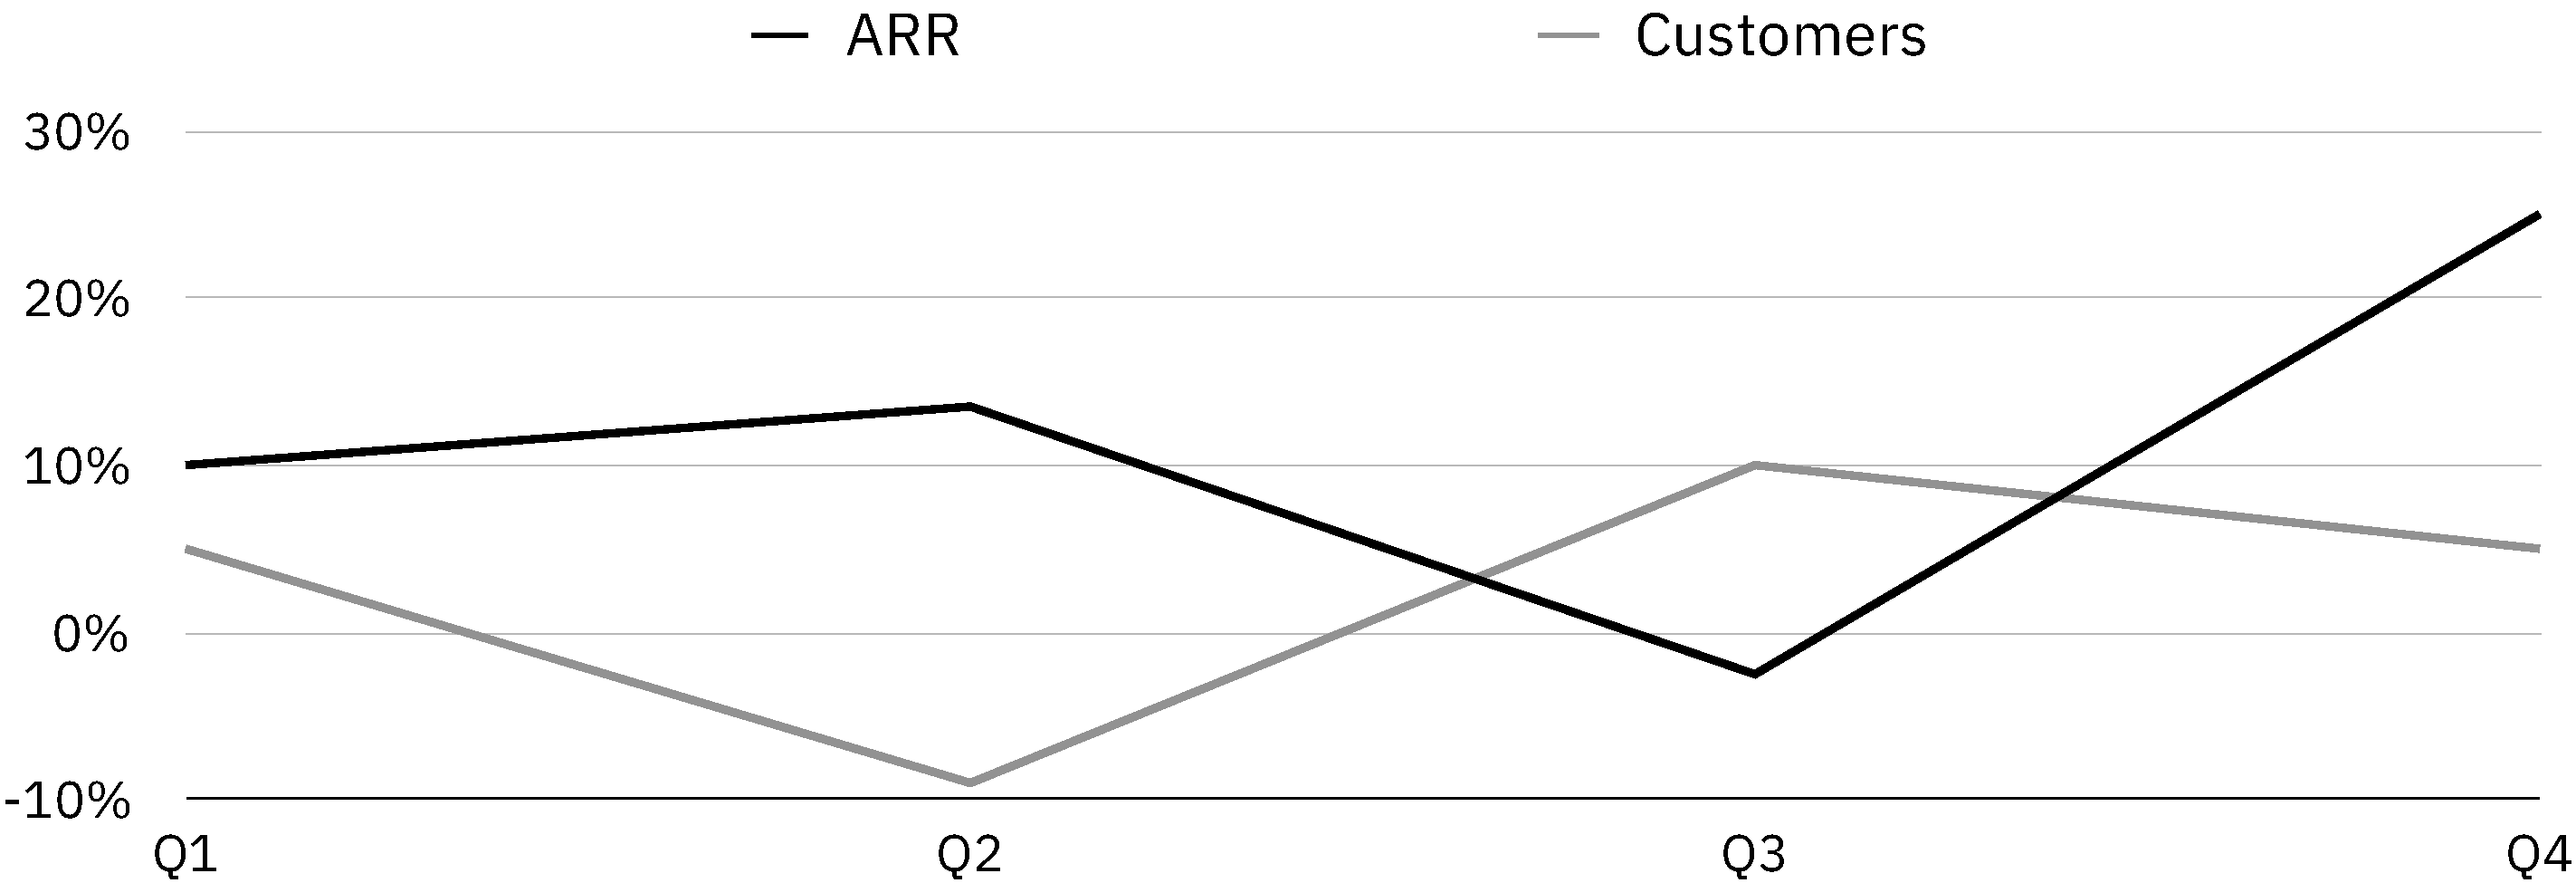
\includegraphics[width=\linewidth]{./include/ARR.pdf}
	\caption{Text block figure caption.}
	\label{fig:example} % Label for referencing this figure in the text automatically
\end{figure}

%------------------------------------------------

\begin{figure*} % Use the figure* environment for full width figures
	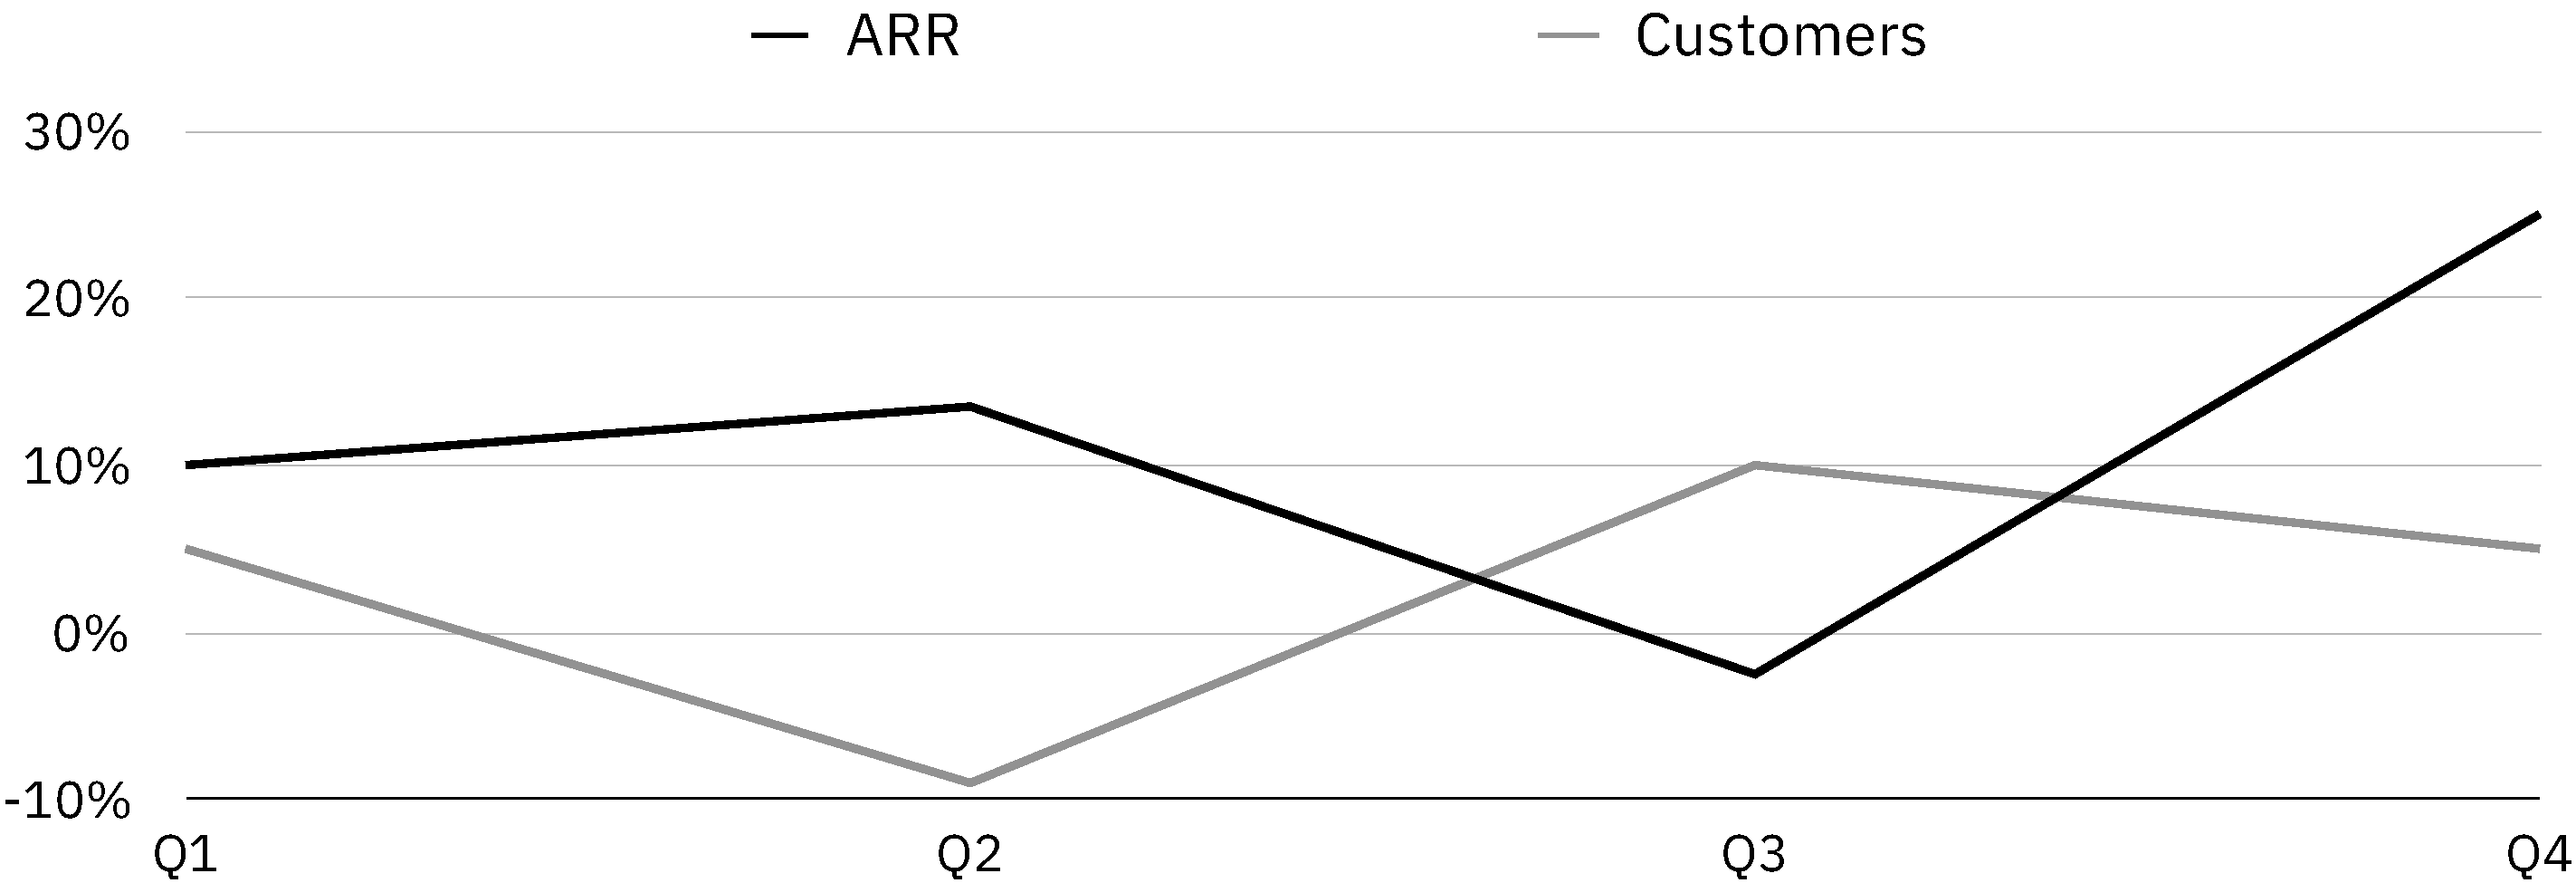
\includegraphics[width=\linewidth]{./include/ARR.pdf}
	\caption{Full width figure caption.}
\end{figure*}

%----------------------------------------------------------------------------------------
%	LISTS
%----------------------------------------------------------------------------------------

\section{List Examples}

\subsection{Bullet Point List}

\nonumsidenote{Bullet point lists can also be created in the margin. For these, we can remove the usual left margin to increase the available horizontal space:\\\medskip \begin{itemize}[leftmargin=*]\item Bullet item one. \item Bullet item two. \item Bullet item three.\end{itemize}}Lorem ipsum dolor sit amet, consectetur adipiscing elit. Praesent porttitor arcu luctus, imperdiet urna iaculis, mattis eros. Pellentesque iaculis odio vel nisl ullamcorper, nec faucibus ipsum molestie. Sed dictum nisl non aliquet porttitor.

\begin{itemize}
	\item First bullet point item
	\begin{itemize}
		\item First indented bullet point item
		\item Second indented bullet point item
		\begin{itemize}
			\item First second-level indented bullet point item
			\item Second second-level indented bullet point item
		\end{itemize}
		\item Third indented bullet point item
	\end{itemize}
	\item Second bullet point item
	\item Third bullet point item
\end{itemize}

Etiam vulputate arcu dignissim, finibus sem et, viverra nisl. Aenean luctus congue massa, ut laoreet metus ornare in. Nunc fermentum nisi imperdiet lectus tincidunt vestibulum at ac elit. Nulla mattis nisl eu malesuada suscipit.

%------------------------------------------------

\subsection{Numbered List}

\nonumsidenote[-2.5cm]{Numbered lists can also be created in the margin. For these, we can remove the usual left margin to increase the available horizontal space:\\\medskip \begin{enumerate}[leftmargin=*]\item Numbered item one. \item Numbered item two. \item Numbered item three.\end{enumerate}}Lorem ipsum dolor sit amet, consectetur adipiscing elit. Praesent porttitor arcu luctus, imperdiet urna iaculis, mattis eros. Pellentesque iaculis odio vel nisl ullamcorper, nec faucibus ipsum molestie. Sed dictum nisl non aliquet porttitor.

\begin{enumerate}
	\item First numbered item
	\begin{enumerate}
		\item First indented numbered item
		\item Second indented numbered item
		\begin{enumerate}
			\item First second-level indented numbered item
			\item Second second-level indented numbered item
		\end{enumerate}
		\item Third indented numbered item
	\end{enumerate}
	\item Second numbered item
	\item Third numbered item
\end{enumerate}

Etiam vulputate arcu dignissim, finibus sem et, viverra nisl. Aenean luctus congue massa, ut laoreet metus ornare in. Nunc fermentum nisi imperdiet lectus tincidunt vestibulum at ac elit. Nulla mattis nisl eu malesuada suscipit.

%------------------------------------------------

\subsection{Description List}

\nonumsidenote{Description lists can also be created in the margin:\\\medskip \begin{description}\item[A1] Description item one. \item[B1] Description item two. \item[C1] Description item three.\end{description}}Lorem ipsum dolor sit amet, consectetur adipiscing elit. Praesent porttitor arcu luctus, imperdiet urna iaculis, mattis eros. Pellentesque iaculis odio vel nisl ullamcorper, nec faucibus ipsum molestie. Sed dictum nisl non aliquet porttitor.

\begin{description}
	\item[Item One] Lorem ipsum dolor sit amet, consectetur adipiscing elit. Praesent porttitor arcu luctus, imperdiet urna iaculis, mattis eros. Pellentesque iaculis odio vel nisl ullamcorper, nec faucibus ipsum molestie.
	\item[Item Two] Sed dictum nisl non aliquet porttitor.
	\begin{description}
		\item[Subitem] Maecenas consectetur metus at tellus finibus condimentum. Proin arcu lectus, ultrices non tincidunt et, tincidunt ut quam. Integer luctus posuere est, non maximus ante dignissim quis.
		\begin{description}
			\item[Subsubitem] Maecenas consectetur metus at tellus finibus condimentum. Proin arcu lectus, ultrices non tincidunt et, tincidunt ut quam. Integer luctus posuere est, non maximus ante dignissim quis.
	\end{description}
	\end{description}
	\item[Item Three] Etiam vulputate arcu dignissim, finibus sem et, viverra nisl. Aenean luctus congue massa, ut laoreet metus ornare in. Nunc fermentum nisi imperdiet lectus tincidunt vestibulum at ac elit. Nulla mattis nisl eu malesuada suscipit.
\end{description}

Etiam vulputate arcu dignissim, finibus sem et, viverra nisl. Aenean luctus congue massa, ut laoreet metus ornare in.

%----------------------------------------------------------------------------------------
%	REFERENCING CITATIONS
%----------------------------------------------------------------------------------------

\section{Referencing Citations}

This statement requires citation \autocite{Smith:2024jd}.

This statement requires multiple citations \autocite{Smith:2024jd, Smith:2023qr}.

This short citation is in the margin\sidecite{Smith:2023qr}.

This long citation is in the margin\fullsidecite{Smith:2024jd}.

This statement has an in-text citation: \textcite{Smith:2024jd}.

%----------------------------------------------------------------------------------------
%	LINKS
%----------------------------------------------------------------------------------------

\section{Link Examples}

This is a URL link: \href{https://www.duckduckgo.com}{DuckDuckGo}.\nonumsidenote{Links can be clicked in the PDF to navigate to the linked website or email address.}

This is a email link: \href{mailto:example@example.com}{example@example.com}.

This is a monospaced URL link: \url{https://duckduckgo.com}.


%----------------------------------------------------------------------------------------
%	CODE
%----------------------------------------------------------------------------------------

\section{Displaying Code}

The block below is a code listing. It displays code in an easy to use way with line numbers for quick reference to specific parts of the code.

\begin{lstlisting}
{
	"city": [
		{
			"id": 1,
			"name": "Toronto",
			"country": "Canada",
			"population": 6200000
		},
		{
			"id": 2,
			"name": "New York",
			"country": "United States of America",
			"population": 8800000
		}
	]
}
\end{lstlisting}

%----------------------------------------------------------------------------------------
%	 REFERENCES/BIBLIOGRAPHY
%----------------------------------------------------------------------------------------

\newpage

\addcontentsline{toc}{section}{Reference List} % Add the bibliography to the table of contents

\begin{twothirdswidth} % Content in this environment to be at two-thirds of the whole page width
	\printbibliography[title=Reference List] % Output the bibliography with a custom section title
\end{twothirdswidth}

%----------------------------------------------------------------------------------------
%	APPENDICES
%----------------------------------------------------------------------------------------

\newpage

\section*{Appendices}

\begin{appendices}

\section{Appendix Section}

Lorem ipsum dolor sit amet, consectetur adipiscing elit. Aliquam auctor mi risus, quis tempor libero hendrerit at. Duis hendrerit placerat quam et semper. Nam ultricies metus vehicula arcu viverra, vel ullamcorper justo elementum. Pellentesque vel mi ac lectus cursus posuere et nec ex. Fusce quis mauris egestas lacus commodo venenatis. Ut at arcu lectus. Donec et urna nunc. Morbi eu nisl cursus sapien eleifend tincidunt quis quis est. Donec ut orci ex. Praesent ligula enim, ullamcorper non lorem a, ultrices volutpat dolor. Nullam at imperdiet urna. Pellentesque nec velit eget euismod pretium.

\section{Appendix Section}

Lorem ipsum dolor sit amet, consectetur adipiscing elit. Aliquam auctor mi risus, quis tempor libero hendrerit at. Duis hendrerit placerat quam et semper. Nam ultricies metus vehicula arcu viverra, vel ullamcorper justo elementum. Pellentesque vel mi ac lectus cursus posuere et nec ex. Fusce quis mauris egestas lacus commodo venenatis. Ut at arcu lectus. Donec et urna nunc. Morbi eu nisl cursus sapien eleifend tincidunt quis quis est. Donec ut orci ex. Praesent ligula enim, ullamcorper non lorem a, ultrices volutpat dolor. Nullam at imperdiet urna. Pellentesque nec velit eget euismod pretium.

\section{Appendix Section}

Lorem ipsum dolor sit amet, consectetur adipiscing elit. Aliquam auctor mi risus, quis tempor libero hendrerit at. Duis hendrerit placerat quam et semper. Nam ultricies metus vehicula arcu viverra, vel ullamcorper justo elementum. Pellentesque vel mi ac lectus cursus posuere et nec ex. Fusce quis mauris egestas lacus commodo venenatis. Ut at arcu lectus. Donec et urna nunc. Morbi eu nisl cursus sapien eleifend tincidunt quis quis est. Donec ut orci ex. Praesent ligula enim, ullamcorper non lorem a, ultrices volutpat dolor. Nullam at imperdiet urna. Pellentesque nec velit eget euismod pretium.

\end{appendices}

%----------------------------------------------------------------------------------------

\end{document}
